\documentclass[tikz]{standalone}
\usetikzlibrary{calc}
\usepackage{tikzpeople}
\begin{document}

\newcommand{\boundellipse}[3]% center, xdim, ydim
{(#1) ellipse (#2 and #3)
}

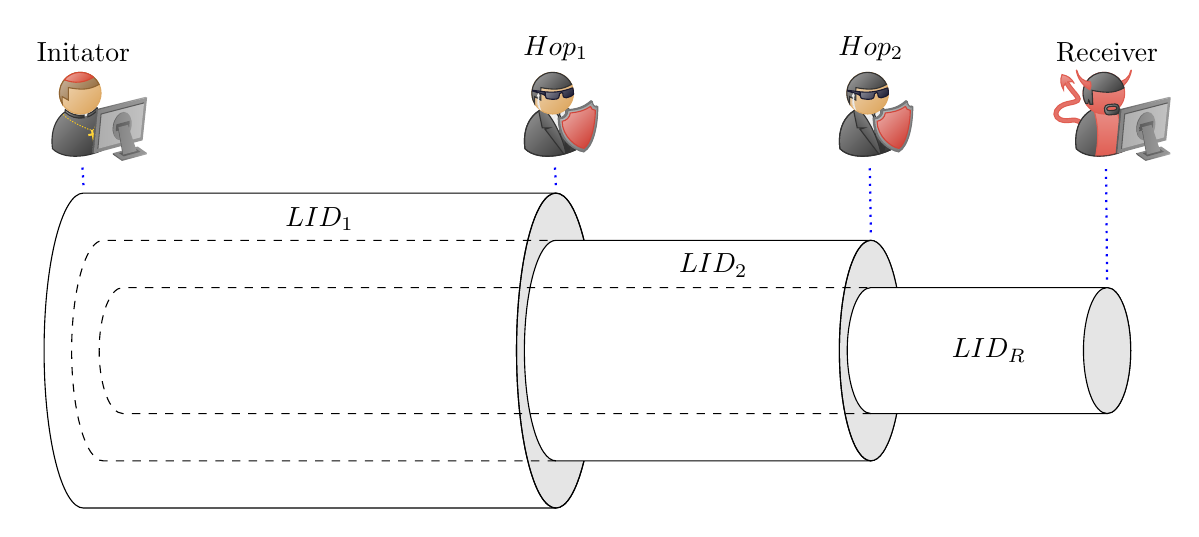
\begin{tikzpicture}
\draw[fill=gray!20] (6,2) ellipse (.5 and 2);
\draw (6,0)--(0,0) arc (270:90:.5 and 2) -- (6,4) arc (90:-90:.5 and 2);

\draw[fill=white] (6,.6)--(10,.6) arc (-90:90:.4 and 1.4) -- (6,3.4) arc (90:270:.4 and 1.4);
\draw[style=dashed] (6,.6)--(.25,.6) arc (270:90:.4 and 1.4) -- (6,3.4);

\draw[fill=gray!20] (10,2) ellipse (.4 and 1.4);
\draw[fill=white] (10,1.2)--(13,1.2) arc (-90:90:.3 and .8) -- (10,2.8) arc (90:270:.3 and .8);
\draw[style=dashed] (10,1.2)--(.5,1.2) arc (270:90:.3 and .8) -- (10,2.8);
\draw[fill=gray!20] (13,2) ellipse (.3 and .8);

\draw (10,3.4) arc (90:270:.4 and 1.4);
\draw (6,4) arc (90:270:.5 and 2);

\node[] at (3,3.67) {$LID_1$};
\node[] at (8,3.08) {$LID_2$};
\node[] at (11.5,2) {$LID_R$};

\node[priest, monitor, minimum size=.8cm, label=above:Initator] at (0, 5) (ot) {};
\node[maninblack, shield, minimum size=.8cm, label=above:$Hop_1$] at (6, 5) (ih1) {};
\node[maninblack, shield, minimum size=.8cm, label=above:$Hop_2$] at (10, 5) (ih2) {};
\node[devil, monitor, minimum size=.8cm, label=above:Receiver] at (13, 5) (r) {};

\draw[color=blue, style=dotted, thick] (0,4.1) -- (ot);
\draw[color=blue, style=dotted, thick] (6,4.1) -- (ih1);
\draw[color=blue, style=dotted, thick] (10,3.5) -- (ih2);
\draw[color=blue, style=dotted, thick] (13,2.9) -- (r);
\end{tikzpicture}
\end{document}